\pdfminorversion=4
\documentclass[10pt]{beamer}\usepackage[]{graphicx}\usepackage[]{color}
%% maxwidth is the original width if it is less than linewidth
%% otherwise use linewidth (to make sure the graphics do not exceed the margin)
\makeatletter
\def\maxwidth{ %
  \ifdim\Gin@nat@width>\linewidth
    \linewidth
  \else
    \Gin@nat@width
  \fi
}
\makeatother

\definecolor{fgcolor}{rgb}{0.345, 0.345, 0.345}
\newcommand{\hlnum}[1]{\textcolor[rgb]{0.686,0.059,0.569}{#1}}%
\newcommand{\hlstr}[1]{\textcolor[rgb]{0.192,0.494,0.8}{#1}}%
\newcommand{\hlcom}[1]{\textcolor[rgb]{0.678,0.584,0.686}{\textit{#1}}}%
\newcommand{\hlopt}[1]{\textcolor[rgb]{0,0,0}{#1}}%
\newcommand{\hlstd}[1]{\textcolor[rgb]{0.345,0.345,0.345}{#1}}%
\newcommand{\hlkwa}[1]{\textcolor[rgb]{0.161,0.373,0.58}{\textbf{#1}}}%
\newcommand{\hlkwb}[1]{\textcolor[rgb]{0.69,0.353,0.396}{#1}}%
\newcommand{\hlkwc}[1]{\textcolor[rgb]{0.333,0.667,0.333}{#1}}%
\newcommand{\hlkwd}[1]{\textcolor[rgb]{0.737,0.353,0.396}{\textbf{#1}}}%

\usepackage{framed}
\makeatletter
\newenvironment{kframe}{%
 \def\at@end@of@kframe{}%
 \ifinner\ifhmode%
  \def\at@end@of@kframe{\end{minipage}}%
  \begin{minipage}{\columnwidth}%
 \fi\fi%
 \def\FrameCommand##1{\hskip\@totalleftmargin \hskip-\fboxsep
 \colorbox{shadecolor}{##1}\hskip-\fboxsep
     % There is no \\@totalrightmargin, so:
     \hskip-\linewidth \hskip-\@totalleftmargin \hskip\columnwidth}%
 \MakeFramed {\advance\hsize-\width
   \@totalleftmargin\z@ \linewidth\hsize
   \@setminipage}}%
 {\par\unskip\endMakeFramed%
 \at@end@of@kframe}
\makeatother

\definecolor{shadecolor}{rgb}{.97, .97, .97}
\definecolor{messagecolor}{rgb}{0, 0, 0}
\definecolor{warningcolor}{rgb}{1, 0, 1}
\definecolor{errorcolor}{rgb}{1, 0, 0}
\newenvironment{knitrout}{}{} % an empty environment to be redefined in TeX

\usepackage{alltt}
%% O comando acima foi necessario porque o PDF nao abria no acrobat do
%% windows, dava o erro 131. Provavelmente devido as figuras em
%% PDF. Agora ele gera um PDF versao 1.4, ao inves da versao 1.5

\usetheme[compress]{PaloAlto}
\usecolortheme{sidebartab} % crane

\usepackage[brazilian]{babel}
\usepackage[T1]{fontenc}
\usepackage[utf8]{inputenc}
\usepackage{graphicx}
\usepackage{hyperref}
\usepackage[scaled]{beramono} % truetype: Bistream Vera Sans Mono
%\usepackage{inconsolata}
\usepackage{xfrac}
\usepackage{tikz}
\usepackage{xcolor}
\usepackage{multirow}
\usepackage{multicol}
\usepackage{tikz}
\usetikzlibrary{arrows, decorations.pathmorphing, backgrounds, fit,
  positioning, calc, trees, plotmarks}

\setbeamertemplate{footline}[frame number] % mostra o numero dos slides
\setbeamertemplate{navigation symbols}{} % retira a barra de navegacao

\usepackage{xspace}
\providecommand{\eg}{\textit{e.g.}\xspace}
\providecommand{\ie}{\textit{i.e.}\xspace}
\providecommand{\R}{\textsf{R}\xspace}
\newcommand{\mb}[1]{\mathbf{#1}}
\newcommand{\bs}[1]{\boldsymbol{#1}}
\providecommand{\E}{\text{E}}
\providecommand{\Var}{\text{Var}}
\providecommand{\DP}{\text{DP}}
\providecommand{\N}{\text{N}}
\theoremstyle{definition}
\newtheorem*{mydef}{Definição}
\newtheorem*{mythm}{Teorema}

\title[Variáveis Aleatórias e Distr. de Probabilidade]{Variáveis
  Aleatórias e Distribuições de Probabilidade}
\author[]{Fernando de Pol Mayer}
\institute[UFPR]{Laboratório de Estatística e Geoinformação (LEG) \\
  Departamento de Estatística (DEST) \\
  Universidade Federal do Paraná (UFPR)}
\date{}
\logo{
\includegraphics[width=1.6cm]{../img/ufpr-logo.png}}
\titlegraphic{
\includegraphics[width=1cm]{../img/CC_by-nc-sa_88x31.png}\\
  \tiny
  \href{https://creativecommons.org/licenses/by-nc-sa/4.0/deed.pt_BR}{Este
    conteúdo está disponível por meio da Licença Creative Commons 4.0
    (Atribuição/NãoComercial/PartilhaIgual)}}

\AtBeginSection[]
{
  \begin{frame}
    \frametitle{Plano de aula}
    \tableofcontents[currentsection]
  \end{frame}
}

\AtBeginSubsection[]
{
  \begin{frame}
    \frametitle{Plano de aula}
    \tableofcontents[currentsection,currentsubsection]
  \end{frame}
}
\IfFileExists{upquote.sty}{\usepackage{upquote}}{}
\begin{document}





\begin{frame}
\maketitle
%\titlepage
\end{frame}

\begin{frame}{Sumário}
\tableofcontents
\end{frame}


\section[Introdução]{Introdução}

\begin{frame}[fragile=singleslide]{Probabilidades}
Já vimos que as probabilidades podem ser definidas de diferentes maneiras:
\begin{itemize}
\item Definição \textbf{clássica}
\item Definição \textbf{frequentista}
\item Definição subjetiva
\item Definição axiomática
\end{itemize}
\end{frame}

\begin{frame}[fragile=singleslide]{Probabilidades}
Vamos relembrar algumas definições \\~\\
 Um experimento, que ao ser realizado sob as mesmas condições
 \underline{\textbf{não}}
 produz os mesmos resultados, é denominado um \textbf{experimento
   aleatório}. Exemplo: lançamento de uma moeda, medir altura, \ldots
 \\~\\
 O conjunto de todos os possíveis resultados de um experimento
 aleatório é denominado \textbf{espaço amostral} ($\Omega$). Pode conter
 um número finito ou infinito de pontos. Exemplo: \{cara, coroa\},
 $\mathbb{R}$, \ldots  \\~\\
 Os elementos do espaço amostral (\textbf{pontos amostrais}) são
 denotados por $\omega$. Exemplo: $\omega_1 = \text{cara}$, $\omega_2 =
 \text{coroa}$. \\~\\
 Todo resultado ou \underline{subconjunto} de resultados de um
 experimento aleatório, é um \textbf{evento}. Exemplo: A = ``sair
 cara'', B = ``sair face par''.
 \end{frame}

\begin{frame}[fragile=singleslide]{Probabilidades}
  \textbf{Axiomas de probabilidade} \\~\\
  Vamos considerar \textbf{probabilidade} como sendo uma função
  $P(\cdot)$ que associa valores numéricos à um evento $A$ do espaço
  amostral, e que satisfaz as seguintes condições \\~\\
  \begin{itemize}
  \item[i)] $P(\Omega) = 1$; $P(\varnothing) = 0$
  \item[ii)] $0 \leq P(A) \leq 1$
  \item[iii)] $P(A \cup B) = P(A) + P(B) \quad\quad
    \text{se, e seomente se}\quad A \cap B = \varnothing$
  \end{itemize}
  \vspace{1em}
  Os axiomas asseguram que as probabilidades podem ser interpretadas
  como \textbf{frequências relativas}.
\end{frame}

\begin{frame}[fragile=singleslide]{Variáveis aleatórias}
  Em probabilidade, uma função $X$ que associa a cada evento do espaço
  amostral um número real $X(\omega) \in \mathbb{R}$, é
  denominada uma \textbf{variável aleatória} (V.A.)\\~\\

  Uma variável aleatória pode ser classificada como \textbf{discreta} ou
  \textbf{contínua}, dependendo do domínio dos valores de $X$.\\~\\

  Exemplo: o número de alunos em uma sala é uma variável aleatória
  (discreta), denotada por $X$ (maiúsculo). Uma observação dessa
  variável é denotada pela respectiva letra minúscula, \eg, $x = 50$
  alunos. \\~\\

  Em geral, denotamos a probabilidade de uma V.A. $X$ assumir determinado
  valor $x$ como
  \begin{equation*}
    P[X] \quad \text{ou} \quad P[X = x]
  \end{equation*}
  %% Exemplo: O peso de uma espécie de peixe é uma variável aleatória
  %% (contínua), denotada por $X$ (maiúsculo). Uma observação dessa
  %% variável é denotada pela letra minúscula, \eg, $x = 5$ kg.

\end{frame}

\begin{frame}[fragile=singleslide]{Variáveis aleatórias}
\begin{block}{Experimento}
Lançamento de duas moedas. $X$ = número de resultados cara (C)
\end{block}
\begin{center}
    %\usetikzlibrary{arrows,decorations.pathmorphing,backgrounds,fit,positioning,calc,trees,plotmarks} %placments

\begin{tikzpicture}
  \draw (0,0) rectangle (3,3) node[above right] at (0,0) {$\Omega$};
  \node[above] at (1.5,3) {elementos de $\Omega$};
  \node (CC) at (2,2) {};
  \node (CK) at (1,2) {};
  \node (KC) at (2,1) {};
  \node (KK) at (1,1) {};
  \node[left, text width=3em, text centered] (arrowstart) at (-2,-2) {valores de $X$};
  \node (arrowend) at (5,-2) {$\mathbb{R}$};
  \draw (CC) circle (2pt) node[above] {CC};
  \draw (KC) circle (2pt) node[above] {RC};
  \draw (CK) circle (2pt) node[above] {CR};
  \draw (KK) circle (2pt) node[above] {RR};
  \draw[->] (arrowstart) -- (arrowend);
  \foreach \x/\y in {0/0,2/1,4/2}
   		\draw (\x,-1.8) -- (\x,-2)
		node[anchor=north] {\y};
  \path[->,>=stealth'] (CC) edge[bend left] (4,-2)
                       (CK) edge[bend left=25] (2,-2)
                       (KC) edge[bend left] (2,-2)
                       (KK) edge[bend left] (0,-2);
\end{tikzpicture}

  \end{center}
\end{frame}

\begin{frame}[fragile=singleslide]{Variáveis aleatórias}
  Dada a realização de um experimento aleatório qualquer, com um certo
  espaço de probabilidade, desejamos estudar a \textbf{estrutura
    probabilística} de quantidades associadas à esse experimento. \\~\\
  Note que antes da realização de um experimento, \textbf{não sabemos seu
  resultado}, entretanto seu espaço de probabilidade pode ser
  previamente estabelecido.\\~\\
  Dessa forma, podemos atribuir probabilidades aos \emph{eventos} desse
  espaço amostral, dando origem ao conceito de \textbf{variável
    aleatória}.
\end{frame}

\begin{frame}[fragile=singleslide]{Distribuições de probabilidade}
Existem diversos \underline{modelos probabilísticos} que
procuram descrever vários tipos de variáveis aleatórias: são as
\textbf{distribuições de probabilidade de variáveis aleatórias}
(discretas ou contínuas). \\~\\

A distribuição de probabilidades de uma V.A. $X$ é, portanto, uma
descrição das probabilidades associadas com os possíveis valores de
$X$. Os valores que $X$ assume determinam o \textbf{suporte} (S) da V.A.
\vspace{1em}
\begin{itemize}
\item \textbf{Variáveis discretas} $\rightarrow$ suporte em um conjunto
  de valores enumeráveis (finitos ou infinitos)
\item \textbf{Variáveis contínuas} $\rightarrow$ suporte em um conjunto
  não enumerável de valores
\end{itemize}
\end{frame}

\begin{frame}[fragile=singleslide]{Distribuições de probabilidade}
Denomina-se de \textbf{distribuição de probabilidade} de alguma variável
aleatória, a \textbf{regra} geral que define a
\begin{itemize}
\item \textbf{função de probabilidade} (fp) (V.A.s discretas), ou a
\item \textbf{função densidade de probabilidade} (fdp) (V.A.s contínuas)
\end{itemize}
para a variável de interesse. \\~\\
Existem muitas distribuições de probabilidade, mas algumas merecem
destaque por sua importância prática.\\~\\
Estas distribuições também são chamadas de \textbf{modelos
  probabilísticos}
\end{frame}

%% Na prática, temos alguma ideia sobre a forma da distribuição, mas
%% não sabemos os valores exatos dos parâmetros. A estimação destes
%% parâmetros é tema de estudo da \textbf{inferência estatística}.

%\section{Variáveis aleatórias}

\section[V.A.s Discretas]{Variáveis aleatórias discretas}

\begin{frame}[fragile=singleslide]{Variáveis aleatórias discretas}
  Uma V.A. é classificada como discreta se assume somente um conjunto
  enumerável (finito ou infinito) de valores. \\~\\
  Exemplos:
  \begin{itemize}
  \item Número de caras ao lançar 3 moedas
  \item Número de chamadas telefônicas que chegam à uma central em 1 hora
  \item Número de votos recebidos
  \item Aprovação no vestibular
  \item Grau de queimadura na pele
  \end{itemize}

\end{frame}

\begin{frame}[fragile=singleslide]{Variáveis aleatórias discretas}
  A \textbf{função de probabilidade} (fp) da VA discreta $X$, que assume
  os valores $x_1, x_2, \ldots, x_n, \ldots$, é a função que atribui
  probabilidades a cada um dos possíveis valores: $\{[x_i, p(x_i)], i =
  1, 2, \ldots\}$, ou seja,
  \begin{equation*}
    P[X = x_i] = p(x_i) = p_i, \quad i = 1, 2, \ldots
  \end{equation*}
  com as seguintes propriedades:
  \vspace{1em}
  \begin{itemize}
  \item[i)] A probabilidade de cada valor deve estar entre 0 e 1
    \begin{equation*}
      0 \leq p(x_i) \leq 1, \quad \forall \, i = 1, 2, \ldots
    \end{equation*}
  \item[ii)] A soma de todas as probabilidades é igual a 1
    \begin{equation*}
    \sum_{i} p(x_i) = 1
  \end{equation*}
  \end{itemize}
  \vspace{1em}
  %% Esperança e variância
  %% \begin{equation*}\small
  %%   \E(X) = \sum_{\forall x \in S} x \cdot P[X = x] \quad \text{e} \quad \Var(X) =
  %%   \sum_{\forall x \in S} (x - \E(X))^2 \cdot P[X = x]
  %% \end{equation*}
  %%   \vspace{1em}
  %% Função de distribuição acumulada
  %% \begin{equation*}\small
  %%   F(x) = \sum_{\forall x' \leq x \in S} P[X = x]
  %% \end{equation*}
\end{frame}

\begin{frame}[fragile=singleslide]{Variáveis aleatórias discretas}
\begin{block}{Experimento}
Lançamento de duas moedas. $X$ = número de resultados cara (C)
\end{block}
\begin{center}
    %\usetikzlibrary{arrows,decorations.pathmorphing,backgrounds,fit,positioning,calc,trees,plotmarks} %placments

\begin{tikzpicture}
  \draw (0,0) rectangle (3,3) node[above right] at (0,0) {$\Omega$};
  \node[above] at (1.5,3) {elementos de $\Omega$};
  \node (CC) at (2,2) {};
  \node (CK) at (1,2) {};
  \node (KC) at (2,1) {};
  \node (KK) at (1,1) {};
  \node[left, text width=3em, text centered] (arrowstart) at (-2,-2) {valores de $X$};
  \node (arrowend) at (5,-2) {$\mathbb{R}$};
  \draw (CC) circle (2pt) node[above] {CC};
  \draw (KC) circle (2pt) node[above] {RC};
  \draw (CK) circle (2pt) node[above] {CR};
  \draw (KK) circle (2pt) node[above] {RR};
  \draw[->] (arrowstart) -- (arrowend);
  \foreach \x/\y in {0/0,2/1,4/2}
   		\draw (\x,-1.8) -- (\x,-2)
		node[anchor=north] {\y};
  \path[->,>=stealth'] (CC) edge[bend left] (4,-2)
                       (CK) edge[bend left=25] (2,-2)
                       (KC) edge[bend left] (2,-2)
                       (KK) edge[bend left] (0,-2);
\end{tikzpicture}

  \end{center}
\end{frame}

\begin{frame}[fragile=singleslide]{Variáveis aleatórias discretas}
  Podemos montar uma tabela de distribuição de frequência para a
  variável aleatória $X$ = número de resultados cara (C)
  \begin{table}[h]
    \centering
    \begin{tabular}{ccc}
      \hline
      $X$ & Frequência ($f_i$) & Frequência relativa ($fr_i$) \\
      \hline
      0 & 1 & 1/4 \\
      1 & 2 & 2/4\\
      2 & 1 & 1/4\\
      \hline
      Total & 4 & 1 \\
      \hline
    \end{tabular}
  \end{table}
  Assim podemos associar a cada valor de $X$ sua \textbf{probabilidade}
  correspondente, como resultado das \textbf{frequências relativas}
  \begin{align*}
    P[X=0] &= 1/4 \\
    P[X=1] &= 2/4 = 1/2 \\
    P[X=2] &= 1/4 \\
  \end{align*}
\end{frame}

\begin{frame}[fragile]{Variáveis aleatórias discretas}
  Dessa forma, a \textbf{distribuição de probabilidade} da variável
  aleatória $X$ = número de resultados cara (C) é a tabela
  \begin{table}[h]
    \centering
    \begin{tabular}{ccc}
      \hline
      $X$ & $P[X = x_i] = p(x_i)$ \\
      \hline
      0 & 1/4 \\
      1 & 1/2\\
      2 & 1/4\\
      \hline
      Total & 1 \\
      \hline
    \end{tabular}
  \end{table}
  Repare que as propriedades da função de probabilidade estão
  satisfeitas:
  \begin{itemize}
  \item[i)] As probabilidades $p(x_i)$ estão entre 0 e 1
  \item[ii)] A soma de todas as probabilidades $p(x_i)$ é 1
  \end{itemize}
  \vspace{1em}
  \pause
  Qual seria a média desta variável aleatória $X$?
\end{frame}

\subsection{Esperança e variância}

\begin{frame}[fragile]{Esperança}
  O \textbf{valor esperado}, ou \textbf{média}, ou \textbf{esperança
    matemática} é uma quantidade utilizada como resumo do comportamento
  de uma V.A. \\~\\
  A média de uma distribuição de probabilidade é a esperança de sua
  variável aleatória. \\~\\
  A esperança de uma V.A. $X$ é obtida multiplicando-se cada valor de $X
  = x_i$, por sua respectiva probabilidade $P[X = x_i]$, e somando os
  produtos resultantes
  \begin{equation*}
    \E(X) = \sum_{i = 1}^{n} x_i \cdot P[X = x_i]
  \end{equation*}
  A esperança é o valor médio que \textbf{esperaríamos} se o experimento
  continuasse sendo repetido várias vezes.
\end{frame}

\begin{frame}[fragile]{Esperança}
  Note que o valor esperado \textbf{pondera} os valores assumidos pela
  V.A. pelas respectivas probabilidades, e não precisa ser um dos
  valores da variável. \\~\\
  A esperança está sempre compreendida entre os valores extremos da
  V.A. \\~\\
  A esperança também é importante pois serve como caracterização de
  diversas distribuições de probabilidade $\rightarrow$
  \textbf{parâmetro}
\end{frame}

\begin{frame}[fragile]{Esperança}
  \textbf{Exemplo:} Determine o valor esperado do número de solicitações
  de empréstimos aprovados por semana ($X$)
  \begin{table}[h]
    \centering
    \begin{tabular}{cc}
      \hline
      $X$ & $P[X = x_i]$ \\
      \hline
      0 & 0,1 \\
      1 & 0,1 \\
      2 & 0,2 \\
      3 & 0,3 \\
      4 & 0,15 \\
      5 & 0,1 \\
      6 & 0,05 \\
      \hline
      Total & 1 \\
      \hline
    \end{tabular}
  \end{table}
\end{frame}

\begin{frame}[fragile]{Esperança}
  \textbf{Exemplo:} Determine o valor esperado do número de solicitações
  de emprétimos aprovados por semana ($X$)
  \begin{table}[h]
    \centering
    \begin{tabular}{ccc}
      \hline
      $X$ & $P[X = x_i]$ & $x_i \cdot P[X=x_i]$ \\
      \hline
      0 & 0,1 & 0 \\
      1 & 0,1 & 0,1 \\
      2 & 0,2 & 0,4 \\
      3 & 0,3 & 0,9 \\
      4 & 0,15 & 0,6  \\
      5 & 0,1 & 0,5\\
      6 & 0,05 & 0,3\\
      \hline
      Total & 1 & 2,8 \\
      \hline
    \end{tabular}
  \end{table}
  \begin{align*}
    \E(X) &= \sum_{i=1}^{7} x_i \cdot P[X = x_i] \\
          &= 0 \cdot 0,1 + 1 \cdot 0,1 + \cdots + 5 \cdot 0,1 + 6 \cdot
          0,05 \\
          &= 2,8
  \end{align*}
\end{frame}

\begin{frame}[fragile]{Variância}
  A variância, como já vimos, dá o grau de dispersão
  dos valores de uma variável aleatória em relação à sua média ou
  esperança $\E(X)$.  A forma geral para o cálculo é
  \begin{align*}
    \Var(X) &= \E[(X - \E(X))^2] \\
            &= \sum_{i=1}^{n} (x_i - \E(X))^2 \cdot P[X=x_i]
  \end{align*}
  No entanto, uma foma mais fácil operacionalmente pode ser deduzida a
  partir da primeira, e temos
  \begin{equation*}
    \Var(X) = \E(X^2) - \E(X)^2
  \end{equation*}
  onde
  \begin{equation*}
    \E(X^2) = \sum_{i = 1}^{n} x_{i}^{2} \cdot P[X = x_i]
  \end{equation*}
\end{frame}

\begin{frame}[fragile]{Variância}
  O \textbf{desvio-padrão} de uma variável aleatória $X$ será portanto
  \begin{equation*}
    \DP(X) = \sqrt{\Var(X)}
  \end{equation*}

  \vspace{1em}
  Assim como a esperança $\E(X)$, a variância $\Var(X)$ também tem
  importância na caracterização de diversas distribuições de
  probabilidade. \\~\\
  Quando se conhece a esperança e a variância de um modelo, ele fica
  totalmente caracterizado, ou seja, sabemos seu formato geral
\end{frame}

\begin{frame}[fragile]{Variância}
  \textbf{Exemplo:} Calcule a variância e o desvio-padrão para  o número
  de solicitações de emprétimos aprovados por semana ($X$)
  \begin{table}[h]
    \centering
    \begin{tabular}{ccccc}
      \hline
      $X$ & $P[X = x_i]$ & $x_i \cdot P[X=x_i]$ & $X^2$ & $x_{i}^{2}
      \cdot P[X=x_i]$ \\
      \hline
      0 & 0,1 & 0 & 0 & 0 \\
      1 & 0,1 & 0,1 & 1 & 0,1 \\
      2 & 0,2 & 0,4 & 4 & 0,8 \\
      3 & 0,3 & 0,9 & 9 & 2,7 \\
      4 & 0,15 & 0,6 & 16 & 2,4  \\
      5 & 0,1 & 0,5 & 25 & 2,5 \\
      6 & 0,05 & 0,3 & 36 & 1,8\\
      \hline
      Total & 1 & 2,8 &   & 10,3 \\
      \hline
    \end{tabular}
  \end{table}
  \begin{small}
  \begin{align*}
    \E(X) &= \textstyle\sum_{i=1}^{7} x_i \cdot P[X = x_i] = 2,8 \\
    \E(X^2) &= \textstyle\sum_{i=1}^{7} x_{i}^2 \cdot P[X = x_i] = 10,3 \\
    \Var(X) &= \E(X^2) - \E(X)^2 \\
            &= 10,3 - 2,8^2 \\
            &= 2,46
  \end{align*}
  \end{small}
\end{frame}

\begin{frame}[fragile]{Variância}
  \textbf{Exercício:} A tabela abaixo apresenta as estimativas de
  retorno para dois investimentos (A e B), em R\$ 1.000,00, sob três
  condições econômicas com diferentes probabilidades
  \begin{table}[h]
    \centering
    \begin{tabular}{lccc}
      \hline
      \textbf{Condição} & \textbf{Probabilidade} & \textbf{Investimento
        A} & \textbf{Investimento B} \\
      \hline
      Recessão & 0,25 & 200 & -100 \\
      Estável & 0,45 & 50 & 100 \\
      Expansão & 0,3 & -100 & 250 \\
      \hline
    \end{tabular}
  \end{table}
  \begin{itemize}
  \item[a)] Calcule a esperança para cada um dos investimentos, para
    verificar qual investimento maximiza o lucro
  \item[b)] Calcule o desvio-padrão para cada um dos investimentos, para
    verificar qual investimento minimiza o risco
  \end{itemize}
\end{frame}

\begin{frame}[fragile]{Esperança e variância}
  \textbf{Propriedades de esperança e variância} \\~\\
  Dada a VA discreta $X$ e a respectiva função de probabilidade $P[X =
  x_i]$, a esperança da função $h(X)$ é dada por
  \begin{equation*}
    \E[h(X)] = \sum_{i = 1}^{n} h(x_{i}) \cdot P[X = x_i]
  \end{equation*}
  \vspace{1em}

  Com isso, pode ser demonstrado que a esperança e a variância possuem
  as seguintes propriedades:
  \begin{equation*}
    \E(aX + b) = a\E(X) + b
  \end{equation*}
  \vspace{1em}
  \begin{equation*}
    \Var(aX + b) = a^2\Var(X)
  \end{equation*}
  \vspace{1em}
  Sendo $a$ e $b$ constantes.
\end{frame}

% \subsubsection{Exercícios}

%%======================================================================
%% Exercício do Bussab, inicio do capitulo 6
%%======================================================================

% \begin{frame}[fragile]{Exercícios}
%   Exercícios 1, 2, 3, 4 do capítulo 6 do livro (pgs. 154--155).
%   \vspace{1em}
%   \begin{itemize}
%   \item[] Pinto, SS; Silva, CS. \textbf{Estatística, Vol I}. Rio Grande:
%     Editora da FURG, 2010. [Cap. 6]
%   \end{itemize}
% \end{frame}

\subsection[Distribuições Discretas]{Distribuições discretas de
  probabilidade}

\begin{frame}[fragile]{Distribuições discretas de probabilidade}
  Os modelos de probabilidade são utilizados para descrever vários
  fenômenos ou situações que encontramos na natureza, ou experimentos
  por nós construídos. \\~\\
  Esses modelos são expressos por uma família de \textbf{distribuições
    de probabilidade} que dependem de um ou mais \textbf{parâmetros}. \\~\\
  O modelo deve representar, na medida do possível, a complexidade que
  envolve o mundo real da população em estudo. \\~\\
  Lembrando que uma V.A. fica completamente caracterizada pela sua
  \textbf{função de probabilidade} e seus parâmetros.
\end{frame}

\subsubsection{Modelo Bernoulli}

\begin{frame}[fragile]{Modelo Bernoulli}
\textbf{Definição:} Uma variável aleatória $X$ segue o modelo Bernoulli
se assume apenas os valores 0 (``fracasso'') ou 1 (``sucesso''). Sua
função de probabilidade é dada por
\begin{equation*}
  P[X = x] = p^x (1-p)^{1-x}, \quad \quad x = 0, 1
\end{equation*}
onde o parâmetro $0 \leq p \leq 1$ é a probabilidade de sucesso. \\~\\
\textbf{Notação:} $X \sim \text{Ber}(p)$  \\~\\
\textbf{Esperança e variância:} $\E(X) = p$ e $\Var(X) = p(1-p)$ \\~\\
\textbf{Exemplo:} lançamento de uma moeda, sexo de um bebê, resultado de
um teste de germinação, \ldots
\end{frame}

\begin{frame}[fragile]{Modelo Bernoulli}
\begin{knitrout}\footnotesize
\definecolor{shadecolor}{rgb}{0.969, 0.969, 0.969}\color{fgcolor}

{\centering 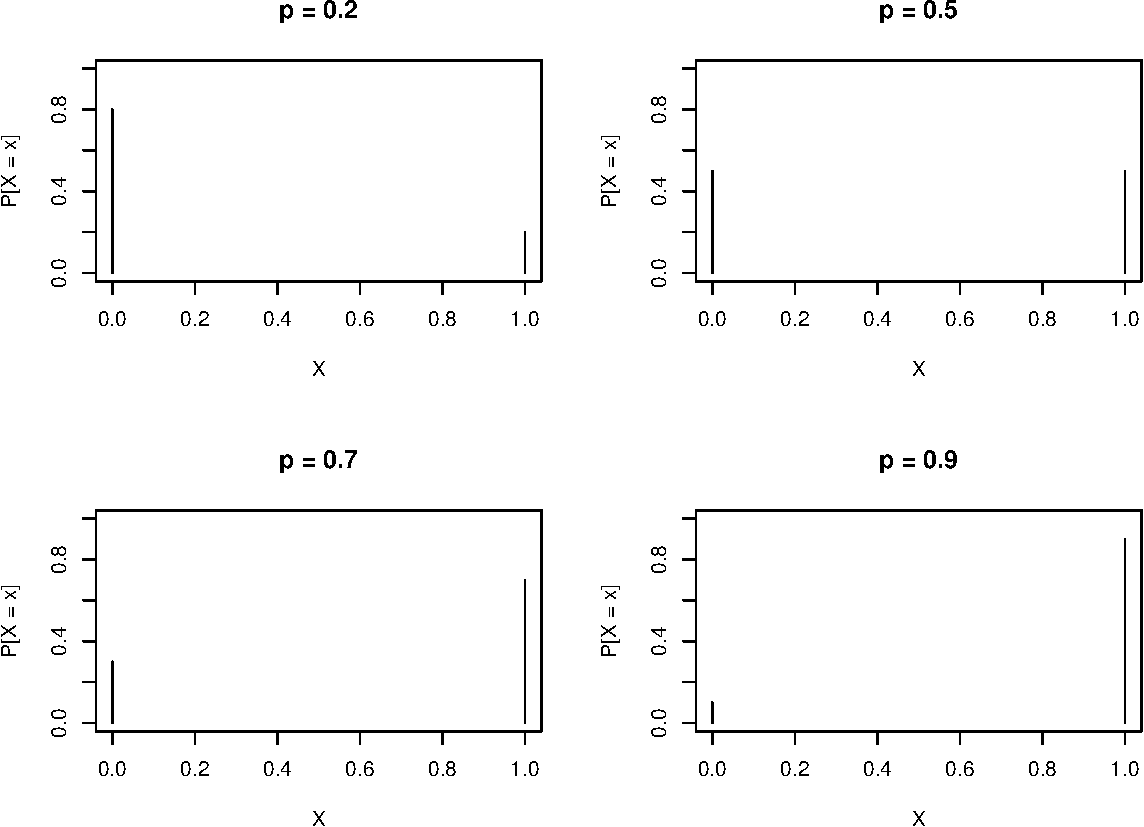
\includegraphics[width=1\textwidth]{figure/unnamed-chunk-1-1} 

}



\end{knitrout}
\end{frame}

\begin{frame}[fragile]{Modelo Bernoulli}
  \textbf{Exemplo:} No lançamento de uma moeda, considere cara como o
  evento de sucesso. Qual a probabilidade de sair cara, sendo que $p =
  1/2$?
  \[ X = \left\{
  \begin{array}{ll}
    1, & \quad \text{cara}\\
    0, & \quad \text{coroa}
  \end{array} \right.\]
Temos que
\begin{table}[h]
  \centering
  \begin{tabular}{ccc}
    \hline
    $X$ & $P[X=x]$ & $p = 1/2$ \\
    \hline
    0 & $1-p$ & $1/2$ \\
    1 & $p$ & $1/2$ \\
    \hline
  \end{tabular}
\end{table}
\end{frame}

\subsubsection{Modelo binomial}

\begin{frame}[fragile]{Modelo binomial}
  \textbf{Definição:} Seja um experimento realizado dentro das seguintes
  condições:
  \begin{itemize}
  \item[i)] São realizados $n$ ``ensaios'' de Bernoulli independentes
  \item[ii)] Cada ensaio só pode ter dois resultados possíveis:
    ``sucesso'' ou ``fracasso''
  \item[iii)] A probabilidade $p$ de sucesso em cada ensaio é constante
  \end{itemize}
  \vspace{1em}
  Vamos associar a V.A. $X$ o número de sucessos em $n$ ensaios de
  Bernoulli. Portanto $X$ poderá assumir os valores $0, 1, \ldots, n$.
\end{frame}

\begin{frame}[fragile]{Modelo binomial}
  Vamos determinar a distribuição de probabilidade de $X$, através da
  probabilidade de um número genérico $x$ de sucessos. \\~\\
  Suponha que ocorram sucessos (1) apenas nas $x$ primeiras provas, e
  fracassos (0) nas $n-x$ provas restantes
  \begin{equation*}
    \underbrace{1,1,1,\ldots, 1}_{x}, \underbrace{0,0,0, \ldots, 0}_{n-x}
  \end{equation*}
  Como as provas são independentes, a probabilidade de ocorrência de $x$
  sucessos em $n$ tentativas é uma extensão do modelo de Bernoulli para
  $n$ ensaios, ou seja,
  \begin{equation*}
    \underbrace{p\cdot p\cdot p \cdots p}_{x} \cdot
    \underbrace{(1-p)\cdot (1-p)\cdot (1-p) \cdots (1-p)}_{n-x}
    = p^x (1-p)^{n-x} %\quad \quad x = 0, 1, \ldots, n
  \end{equation*}
\end{frame}

\begin{frame}[fragile]{Modelo binomial}
  Porém, o evento: ``$x$ sucessos em $n$ provas'' pode ocorrer de
  diferentes maneiras (ordens) distintas, todas com a mesma
  probabilidade. \\~\\
  Como o número de ordens é o número de combinações de $n$ elementos
  tomados $x$ a $x$, então a probabilidade de ocorrerem $x$ sucessos em
  $n$ provas de Bernoulli será então a distribuição binomial, dada por
  \begin{equation*}
    P[X = x] = \binom{n}{x} p^x (1-p)^{n-x}, \quad \quad x = 0, 1, \ldots, n
  \end{equation*}
  onde
  \begin{equation*}
    \binom{n}{x} = \frac{n!}{x!(n-x)!}
  \end{equation*}
  é o \textbf{coeficiente binomial}, que dá o número total de
  combinações possíveis de $n$ elementos, com $x$ sucessos.
\end{frame}

\begin{frame}[fragile]{Modelo binomial}
  \textbf{Notação:} $X \sim \text{bin}(n,p)$ \\~\\
  \textbf{Esperança e variância:} $\E(X) = np$ e $\Var(X) = np(1-p)$ \\~\\
  \textbf{Exemplo:} número de caras no lançamento de 20 moedas, número de
  meninos entre 10 bebês, número de sementes germinadas em 100 sementes,
  \ldots
\end{frame}

\begin{frame}[fragile]{Modelo binomial}
\begin{knitrout}\footnotesize
\definecolor{shadecolor}{rgb}{0.969, 0.969, 0.969}\color{fgcolor}

{\centering 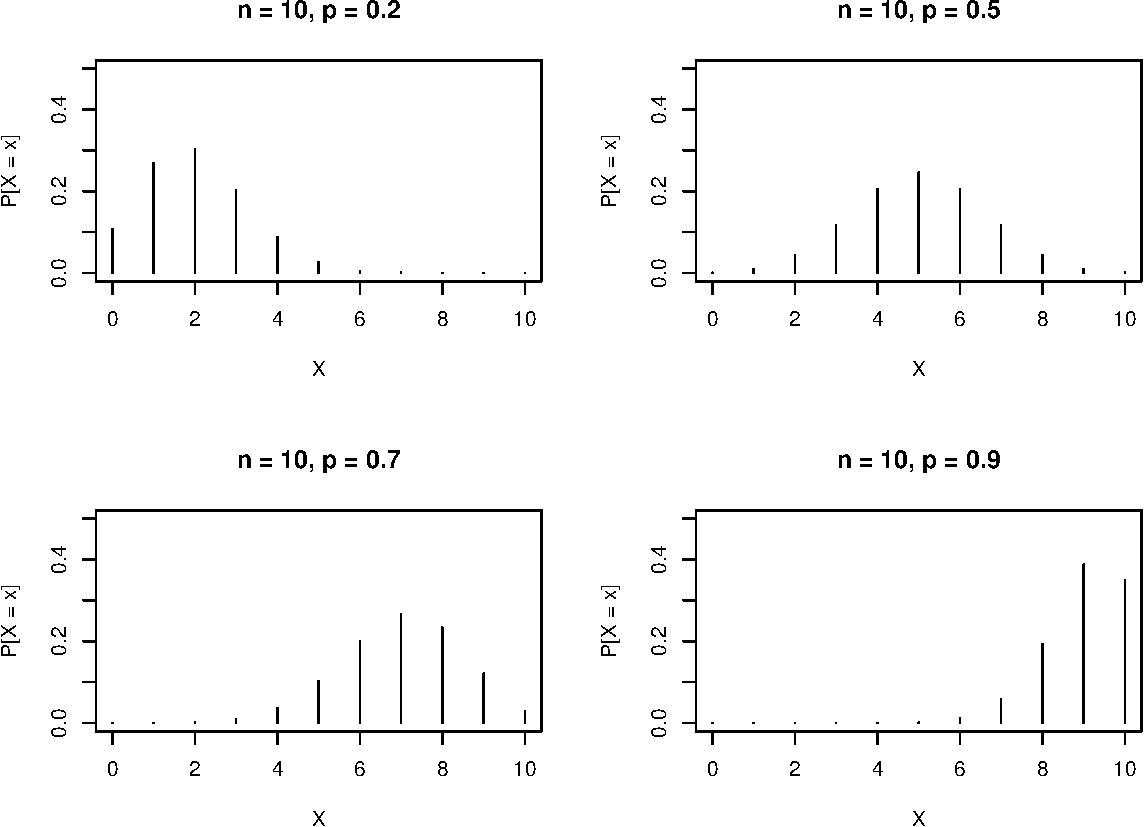
\includegraphics[width=1\textwidth]{figure/unnamed-chunk-2-1} 

}



\end{knitrout}
\end{frame}

\begin{frame}[fragile]{Modelo binomial}
  \textbf{Exemplo:} Determine a probabilidade de ocorrer exatamente duas
  caras no lançamento de três moeda. \\~\\
  Experimento binomial:
  \begin{itemize}
  \item tentativas independentes
  \item dois resultados possíveis: cara (sucesso), coroa (fracasso)
  \item probabilidade de sair cara é constante
  \end{itemize} \pause
  \vspace{1em}
  \textbf{Exemplo:} Suponha que no exemplo anterior fossem lançadas 10
  moedas, qual a probabilidade de ocorrerem exatamente duas caras?
\end{frame}

\begin{frame}[fragile]{Modelo binomial}
  \textbf{Exemplos}
  \vspace{1em}
  \begin{enumerate}
  \item Numa empresa, 40\% dos contratos são pagos em dia. Qual a
    probabilidade de que, entre 12 contratos, três ou menos sejam pagos
    em dia?
  \item Numa criação de coelhos, 40\% são machos. Qual a probabilidade
    de que nasçam pelo menos 2 coelhos machos num dia em que nasceram 20
    coelhos?
  \end{enumerate}
\end{frame}

\begin{frame}[fragile]{Modelo binomial}
  \textbf{Esperança e variância} \\~\\
  Como vimos, a esperança e a variância de uma V.A. $X$ que possui
  distribuição binomial, são dadas por
  \begin{equation*}
    \E(X) = np \quad \text{e} \quad \Var(X) = np(1-p)
  \end{equation*}
  Portanto, conhecendo os parâmetros $n$ e $p$, podemos agora utilizar
  estas definições para calcular a esperança e a variância de uma
  V.A. $X$ binomial, sem a necessidade de realizar os cálculos pelas
  equações gerais de esperança e variância.
\end{frame}

\begin{frame}[fragile]{Modelo binomial}
  \textbf{Exemplo:} Sabe-se que a eficiência de uma vacina é de 70\%. Um
  grupo de 20 indivíduos vacinados é observado e testes são realizados
  para verificar se a imunização foi efetiva.\\~\\
  Seja a V.A. $X$ = número de indivíduos imunizados. Calcule o número
  esperado de indivíduos imunizados, e o desvio padrão.
\end{frame}

% \subsubsection{Exercícios}

%%======================================================================
%% Exercícios do Morettin, LG - cap 4, pgs 109--113
%%======================================================================

% \begin{frame}[fragile]{Exercícios}
%   Exercícios distribuição binomial: 1, 4, 7, 8, do capítulo 7 do
%   livro (pgs. 167--169).
%   \vspace{1em}
%   \begin{itemize}
%   \item[] Pinto, SS; Silva, CS. \textbf{Estatística, Vol I}. Rio Grande:
%     Editora da FURG, 2010. [Cap. 7]
%   \end{itemize}
% \end{frame}

%% \begin{frame}[fragile=singleslide]{Modelo Binomial}
%% \textbf{Exemplo:} Considere o lançamento de uma moeda honesta ($p =
%% 0,5$) 20 vezes ($n=20)$. O gráfico desta distribuição Binomial($n =
%% 20, p = 0,5$) é
%% <<pdfcrop=TRUE>>=
%% plot(0:20, dbinom(x = 0:20, size = 20, prob = .5), type = "h",
%%      xlab = "X", ylab = "P[X = x]")
%% @

%% <<eval=FALSE, echo=FALSE>>=
%% # Densidade de probabilidade
%% dbinom(x = 2, size = 20, prob = .5)
%% # Probabilidade acumulada P[X <= 2]
%% pbinom(q = 2, size = 7, prob = .3)
%% # Quantil
%% qbinom(p = 0.4, size = 7, prob = .3)
%% @
%% \end{frame}

\subsubsection{Modelo Poisson}

\begin{frame}[fragile]{Modelo Poisson}
  \textbf{Definição:} Seja um experimento realizado nas seguintes
  condições: \\~\\
  \begin{itemize}
  \item[i)] As ocorrências são independentes
  \item[ii)] As ocorrências são aleatórias
  \item[iii)] A variável aleatória $X$ é o número de ocorrências de um
    evento \textbf{ao longo de algum intervalo} (de tempo ou espaço)
  \end{itemize}
  \vspace{1em}
  % Denominamos esse experimento de \textbf{processo de Poisson}. \\~\\
  Vamos associar a V.A. $X$ o número de ocorrências em um
  intervalo. Portanto $X$ poderá assumir os valores $0, 1, \ldots,$ (sem
  limite superior).
\end{frame}

\begin{frame}[fragile]{Modelo Poisson}
  Considere então agora que o fenômeno de interesse é observado em um
  intervalo \textbf{contínuo} (tempo, espaço, \ldots), de tamanho $t$.
  \\~\\
  O número de eventos que ocorrem no intervalo fixo $[0,t)$ é uma
  variável aleatória $X$ (``número de sucessos''). \\~\\
  Podemos então inicialmente tentar aproximar esses eventos à um ensaio
  de Bernoulli, criando $n$ subintervalos muito pequenos, de forma que
  este processo satisfaça as seguintes condições:
\end{frame}

\begin{frame}[fragile]{Modelo Poisson}
  \begin{enumerate}
  \item[i)] Em um período de tempo muito curto, somente 1 ou 0 eventos
    podem ocorrer (dois ou mais eventos são impossíveis)
  \item[ii)] O valor esperado de sucessos, $np$, é constante para
    qualquer tamanho de intervalo. Chamaremos essa constante de $\lambda
    = np$. Dessa forma, a probabilidade de sucesso de um evento será $p
    = \lambda/n$.
  \item[iii)] Cada subintervalo é um ensaio de Bernoulli independente.
  \end{enumerate}
  \vspace{1em}
  Um experimento que satisfaça estas condições é chamado de
  \textbf{processo de Poisson}.
\end{frame}

\begin{frame}[fragile]{Modelo Poisson}
  Note que se estas condições forem satisfeitas, se continuarmos
  aumentando o número de subintervalos ($n$), então a probabilidade $p$
  deverá diminuir para que $\lambda = np$ permaneça constante. \\~\\
  Dessa forma, estamos interessados em determinar a distribuição da VA
  $X ~ \sim \text{bin}(n, p = \lambda/n)$ no limite quando $n \to
  \infty$ e $p \to 0$, ou seja,
  \begin{align*}
    P[X = x] &= \lim_{n \to \infty} \binom{n}{x} p^x (1-p)^{n-x} \\
     &= \lim_{n \to \infty} \frac{n!}{x!(n-x)!} \left( \frac{\lambda}{n} \right)^x
       \left( 1 - \frac{\lambda}{n}  \right)^{n-x}
  \end{align*}
\end{frame}

\begin{frame}[fragile]{Modelo Poisson}
  Dessa forma, pode-se mostrar que
  \begin{align*}
    P[X = x] &= \lim_{n \to \infty} \frac{n!}{x!(n-x)!}
               \left( \frac{\lambda}{n} \right)^x
               \left( 1 - \frac{\lambda}{n}  \right)^{n-x} \\
             &\cong \frac{e^{-\lambda} \lambda^x}{x!}
  \end{align*}
  Que é chamado \textbf{modelo de Poisson} com parâmetro $\lambda$, e
  \begin{equation*}
  \E(X) = \lambda = \Var(X)
\end{equation*}
\end{frame}

\begin{frame}[fragile]{Modelo Poisson}
  Nesse caso, $\lambda$ é o número esperado de sucessos em uma unidade
  de tempo específica. \\~\\
  Frequentemente estamos interessados no valor esperado ou na
  probabilidade em um intervalo contínuo $t$ qualquer. Nesse caso, a
  esperança e a variância serão
  \begin{align*}
    \E(X) &= \lambda t = \mu \\
    \Var(X) &= \lambda t
  \end{align*}
  \vspace{1em}

  Portanto, o modelo Poisson mais geral pode ser definido como a seguir:
\end{frame}

\begin{frame}[fragile]{Modelo Poisson}
  Uma V.A. $X$ segue o modelo de Poisson se surge a partir de um
  processo de Poisson, e sua \textbf{função de probabilidade} for dada
  por
  \begin{equation*}
    P[X = x] = \frac{e^{-\mu} \mu^x}{x!}, \quad \quad x = 0, 1, \ldots
  \end{equation*}
  onde
  \begin{equation*}
    \mu = \lambda \cdot t
  \end{equation*}
  O parâmetro $\mu$ indica a taxa de ocorrência ($\lambda$) por unidade
  de medida ($t$), ou seja, %(volume, área, $\ldots$)
  \begin{equation*}
    \lambda = \text{taxa de ocorrência} \quad \text{e} \quad t =
    \text{intervalo de tempo ou espaço}
  \end{equation*}
  %% \textbf{Esperança e variância:} $\E(X) = \mu$ e $\Var(X) = \mu$
\end{frame}

\begin{frame}[fragile]{Modelo Poisson}
  A distribuição de Poisson é utilizada para descrever
  a probabilidade do \textbf{número de ocorrências} em um \textbf{intervalo
  contínuo} (de tempo ou espaço). \\~\\
  No caso da distribuição binomial, a variável de interesse era o número
  de sucessos em um \textbf{intervalo discreto} ($n$ ensaios de
  Bernoulli). \\~\\
  A unidade de medida (tempo ou espaço) é uma variável contínua, mas a
  \textsf{variável aleatória}, o \textbf{número de ocorrências}, é
  discreta.
\end{frame}


\begin{frame}[fragile]{Modelo Poisson}
  % \small
  % A distribuição de Poisson também pode ser pensada como uma aproximação
  % para a distribuição binomial, quando o número de ensaios de Bernoulli
  % for muito grande ($n \rightarrow \infty$) e a probabilidade de sucesso
  % for muito pequena ($p \rightarrow 0$), ou seja,
  % \begin{align*}
  %   P[X=x] &= \lim_{n \rightarrow \infty} \binom{n}{x} p^x (1-p)^{n-x} \\
  %          &\cong \frac{e^{-\mu} \mu^x}{x!} \quad \text{com} \quad \mu
  %          = np
  % \end{align*}
  A distribuição de Poisson difere da distribuição binomial
  em dois aspectos fundamentais: \\~\\
  \begin{enumerate}
  \item A distribuição binomial é afetada pelo tamanho $n$ da amostra, e
    pela probabilidade $p$ de sucesso. A distribuição de Poisson é
    afetada apenas pela média $\mu$.
  \item Na distribuição binomial, os valores possíveis da V.A. $X$ são
    $0, 1, \ldots, n$. Na distribuição de Poisson, a V.A. $X$ tem
    valores possíveis $0, 1, \ldots$, sem nenhum limite superior.
  \end{enumerate}
\end{frame}

\begin{frame}[fragile]{Modelo Poisson}
  \textbf{Notação:} $X \sim \text{Pois}(\mu)$ \\~\\
  \textbf{Esperança e variância:} $\E(X) = \mu = \Var(X)$ \\~\\
  \textbf{Exemplos}
  \begin{itemize}
  \item carros que passam por um cruzamento por minuto, durante uma
    certa hora do dia
  \item erros tipográficos por página, em um material impresso
  \item defeitos por unidade (m, m$^2$, m$^3$, \ldots) por peça
    fabricada
  \item colônias de bactérias numa dada cultura, em uma plaqueta de
    microscópio
  \item mortes por ataque do coração por ano, em uma cidade
  \end{itemize}
\end{frame}

\begin{frame}[fragile]{Modelo Poisson}
  Exemplo: suponha que em um determinado processo de fabricação de
  tecidos ocorra, em média, uma falha a cada 400 metros. Portanto
  \begin{equation*}
    \lambda = \frac{1}{400} = 0,0025 \,
    \frac{\text{falhas}}{\text{metro}}
  \end{equation*}
  Suponha que queremos estudar o número de falhas que aparecerão em 1000
  metros de tecido ($t$). Esse número será uma V.A. $X$ com distribuição
  de Poisson, e o número médio de falhas será então
  \begin{align*}
    \E(X) &= \mu \\
          &= \lambda \cdot t \\
          &= 0,0025 \cdot 1000 \\
          &= 2,5 \, \text{falhas/1000 m}
  \end{align*}
\end{frame}

\begin{frame}[fragile]{Modelo Poisson}
\begin{knitrout}\footnotesize
\definecolor{shadecolor}{rgb}{0.969, 0.969, 0.969}\color{fgcolor}

{\centering 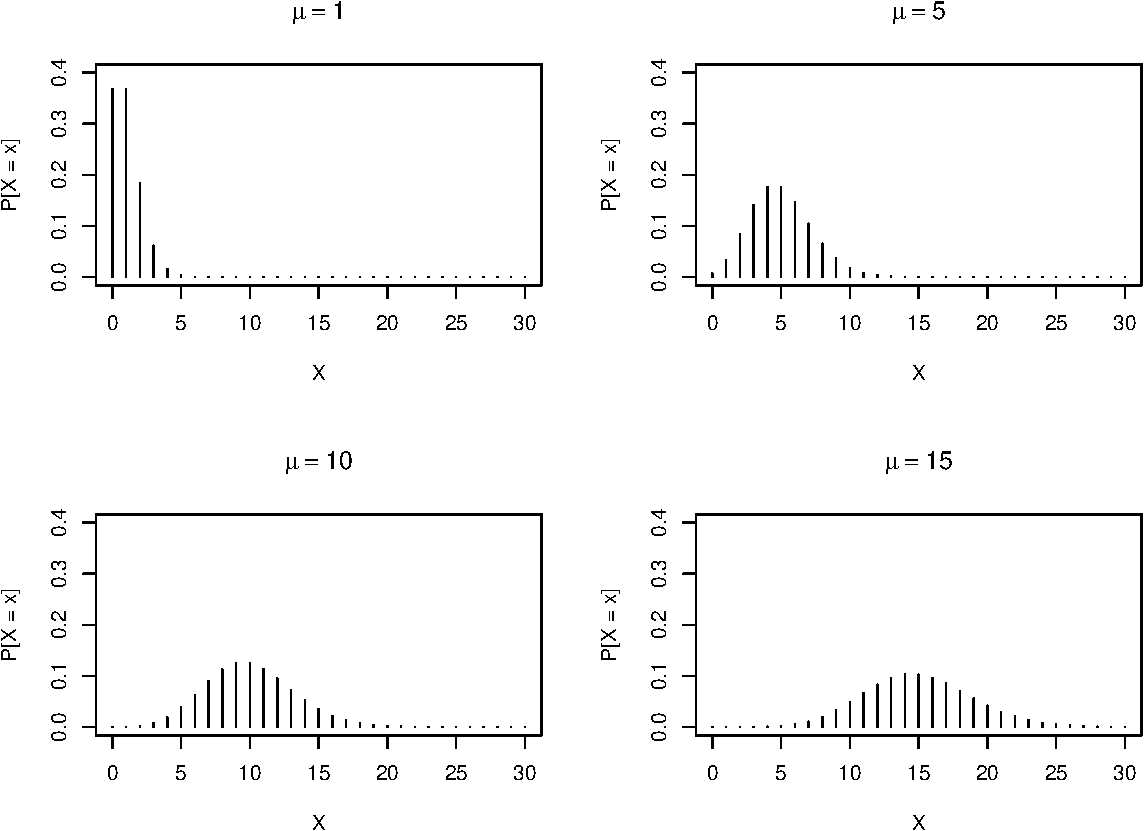
\includegraphics[width=1\textwidth]{figure/unnamed-chunk-3-1} 

}



\end{knitrout}
\end{frame}

\begin{frame}[fragile]{Modelo Poisson}
  \textbf{Exemplo:} As chamadas telefônicas chegam a uma delegacia de
  polícia à uma taxa de 8 chamadas por hora, em dias úteis.
  \begin{itemize}
  \item[a)] Quantas chamadas de emergência são esperadas em um período
    de 15 minutos?
  \item[b)] Qual a probabilidade de nenhuma chamada em um período de 15
    minutos?
  \item[c)] Qual a probabilidade de ocorrer pelo menos duas chamadas no
    período de 15 minutos?
  \item[d)] Qual a probabilidade de ocorrer exatamente duas chamadas em
    20 minutos?
  \end{itemize}
\end{frame}

\begin{frame}[fragile]{Modelo Poisson}
  \textbf{Exemplo:} Suponha que 150 erros de impressão são distribuídos
  aleatoriamente em um livro de 200 páginas. Encontre a probabilidade de
  que em 2 páginas contenham:
  \begin{itemize}
  \item[a)] nenhum erro de impressão
  \item[b)] três erros de impressão
  \item[c)] um ou mais erros de impressão
  \end{itemize}
\end{frame}

%% \begin{frame}[fragile=singleslide]{Modelo Poisson}
%% \textbf{Exemplo:} Suponha que o número de particulas alfa emitidas por
%% minuto seja uma V.A. que segue o modelo de Poisson, com parâmetro
%% 5. Isto é, a taxa média de emissões é de 5 partículas por minuto. O
%% gráfico da distribuição Poisson($\lambda = 5$) é
%% <<pdfcrop=TRUE>>=
%% plot(0:20, dpois(x = 0:20, lambda = 5), type = "h",
%%      xlab = "X", ylab = "P[X = x]")
%% @
%% <<eval=FALSE, echo=FALSE>>=
%% # Densidade de probabilidade para x = 2 com Poisson(1.8)
%% dpois(x = 2, lambda = 1.8)
%% # Probabilidade acumulada P[X <= 3]
%% ppois(q = 3, lambda = 1.8)
%% @
%% \end{frame}

% \subsubsection{Exercícios}

%%======================================================================
%% Exercícios do Morettin, LG - cap 4, pgs 109--113
%%======================================================================

% \begin{frame}[fragile]{Exercícios}
%   Exercícios distribuição Poisson: 2, 5, 6, 9, 10, do capítulo 7 do
%   livro (pgs. 167--169).
%   \vspace{1em}
%   \begin{itemize}
%   \item[] Pinto, SS; Silva, CS. \textbf{Estatística, Vol I}. Rio Grande:
%     Editora da FURG, 2010. [Cap. 7]
%   \end{itemize}
% \end{frame}

\section[V.A.s Contínuas]{Variáveis aleatórias contínuas}

\begin{frame}[fragile]{Variáveis aleatórias contínuas}
  Uma V.A. é classificada como contínua se assume valores em qualquer
  intervalo dos números reais, ou seja, um conjunto de valores não
  enumerável. Dessa forma, não é possível atribuir probabilidades para
  um ponto específico, apenas para intervalos da reta. \\~\\
  Exemplos:
  \begin{itemize}
  \item Peso de animais
  \item Tempo de falha de um equipamento eletrônico
  \item Altura da maré em uma hora específica
  \item Salinidade da água do mar
  \item Retorno financeiro de um investimento
  \end{itemize}
\end{frame}

\begin{frame}[fragile]{Variáveis aleatórias contínuas}
  Não podemos atribuir probabilidades à valores específicos, pois há uma
  quantidade \textbf{não enumerável} (infinita) de valores em um
  ponto. \\~\\
  Atribuimos probabilidades à intervalos de valores,
  por meio de uma \textbf{função}. Portanto, as probabilidades são
  representadas por áreas.
\begin{knitrout}\footnotesize
\definecolor{shadecolor}{rgb}{0.969, 0.969, 0.969}\color{fgcolor}

{\centering 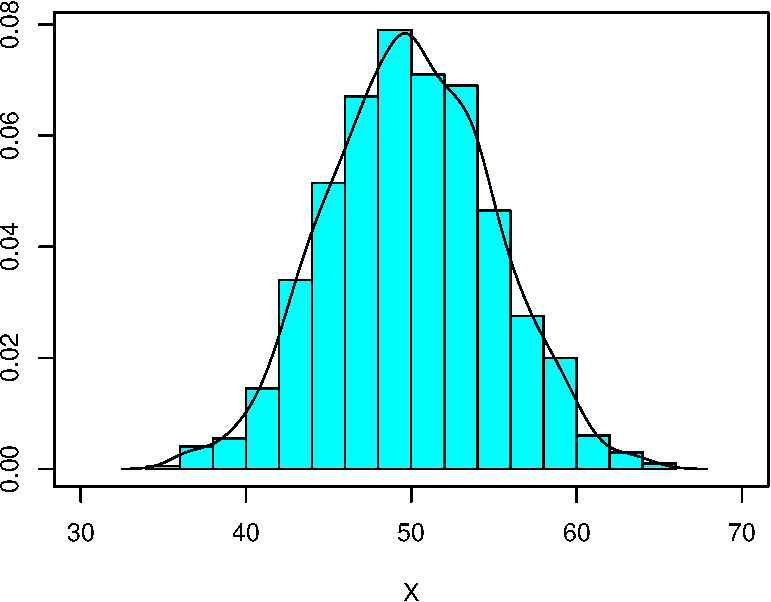
\includegraphics[width=.7\textwidth]{figure/unnamed-chunk-4-1} 

}



\end{knitrout}
\end{frame}

\begin{frame}[fragile]{Variáveis aleatórias contínuas}
  A \textbf{função densidade de probabilidade} (fdp) atribui
  probabilidades à intervalos de valores do tipo $[a,b]$, e é definida
  por
  \begin{equation*}
    P[a < x < b] = \int_{a}^{b} f(x) dx
  \end{equation*}
  com as seguintes propriedades
  \begin{itemize}
  \item[i)] É uma função não negativa
    \begin{equation*}
      f(x) \geq 0
    \end{equation*}
  \item[ii)] A área total sob a curva deve ser igual a 1
    \begin{equation*}
      \int_{-\infty}^{+\infty} f(x) dx = 1
    \end{equation*}
  \end{itemize}
\end{frame}

%% IMPORTANTE: aqui poderia ser dado um exemplo como o do livro do
%% dantas (que eh o mesmo que esta no meu caderno de concurso), mas como
%% envolve integral nao vou colocar para esse curso

%% \begin{frame}[fragile=singleslide]{Variáveis aleatórias contínuas}
%%   A \textbf{função densidade de probabilidade} (fdp) atribui
%%   probabilidades à intervalos de valores do tipo $[a,b]$, e é definida
%%   por
%%   \begin{equation*}
%%    P[a < x < b] = \int_{a}^{b} f(x) dx
%%   \end{equation*}
%%   com as seguintes propriedades
%%   \begin{itemize}\small
%%   \item[i)] $f(x) \geq 0 \quad \forall\, x \in S$
%%   \item[ii)] $\int_{\forall x \in S} f(x) dx = 1$
%%   \end{itemize}
%%   \vspace{1em}
%%     Esperança e variância
%%   \begin{equation*}\small
%%     \E(X) = \int_{\forall x \in S} x \cdot f(x)dx \quad \text{e} \quad \Var(X) =
%%     \int_{\forall x \in S} (x - \E(X))^2 \cdot f(x)dx
%%   \end{equation*}
%%     \vspace{1em}
%%   Função de distribuição acumulada
%%   \begin{equation*}\small
%%     F(x) = \int_{\forall x' \leq x \in S} f(x)dx
%%   \end{equation*}
%% \end{frame}

\begin{frame}[fragile]{Variáveis aleatórias contínuas}
  \textbf{Observações:} \\~\\
  \begin{enumerate}
  \item $P[X=x] = 0$, portanto:
    \begin{equation*}
    P[a \leq X \leq b] = P[a < X \leq b] =
    P[a \leq X < b] = P[a < X < b]
  \end{equation*}
  \item Qualquer função $f(\cdot)$ que seja não negativa e cuja área
    total sob a curva seja igual à unidade caracterizará uma VA
    contínua.
  \item $f(x)$ \emph{não} representa a probabilidade de ocorrência de
    algum evento, A área sobb  curva entre dois pontos é que fornecerá a
    probabilidade.
  \end{enumerate}
\end{frame}

\begin{frame}[fragile]{Exemplo}
  Seja a função:
  \[
    f(x)=
    \begin{cases}
      1,5 x^2, & \text{se } -1 \leq x \leq 1 \\
      0,              & \text{caso contrário}
    \end{cases}
  \]
  \begin{enumerate}
  \item Verifique se essa função é uma fdp.
  \item Calcule:
    \begin{enumerate}
    \item $P[X > 0]$
    \item $P[X > 0,5]$
    \item $P[-0,5 \leq X \leq 0,5]$
    \item $P[X < -2]$
    \item $P[X < 0,5]$
    \item $P[X < 0 \cup X > 0,5]$
    \end{enumerate}
  \end{enumerate}
\end{frame}

\subsection{Esperança e variância}

\begin{frame}[fragile]{Esperança}
  A esperança de uma V.A. contínua tem o mesmo sentido e interpretação
  da esperança de uma V.A. discreta: é a \textbf{média} ou \textbf{valor
    esperado} da V.A. \\~\\
  A esperança de uma V.A. contínua é obtida através da integral do
  produto de $x$ com a função $f(x)$, no intervalo definido pelo suporte
  da V.A. De maneira geral,
  \begin{equation*}
    \E(X) = \int_{-\infty}^{+\infty} x \cdot f(x) dx
  \end{equation*}
\end{frame}

\begin{frame}[fragile]{Variância}
  A variância, como já vimos, dá o grau de dispersão
  dos valores de uma variável aleatória em relação à sua média ou
  esperança $\E(X)$.  A forma geral para o cálculo em V.A.s contínuas é
  \begin{align*}
    \Var(X) &= \E[(X -  \E(X))^2] \\
      &= \int_{-\infty}^{+\infty} [x - \E(X)]^2 \cdot f(x) dx
  \end{align*}
  No entanto, assim como para V.A.s discretas, uma foma mais fácil
  operacionalmente pode ser deduzida a partir da primeira, e temos
  \begin{equation*}
    \Var(X) = \E(X^2) - \E(X)^2
  \end{equation*}
  onde
  \begin{equation*}
    \E(X^2) = \int_{-\infty}^{+\infty} x^2 \cdot f(x) dx
  \end{equation*}
\end{frame}

%% AQUI tambem poderia dar um exemplo com integrais

\begin{frame}[fragile]{Exemplo}
  Seja a função:
  \[
    f(x)=
    \begin{cases}
      1,5 x^2, & \text{se } -1 \leq x \leq 1 \\
      0,              & \text{caso contrário}
    \end{cases}
  \]
  \begin{enumerate}
  \item Calcule a esperança, a variância, e o desvio-padrão.
  \end{enumerate}
\end{frame}


\subsection[Distribuições Contínuas]{Distribuições contínuas de
  probabilidade}

\begin{frame}[fragile]{Distribuições contínuas de probabilidade}
  Existem diversos modelos contínuos de probabilidade. Alguns deles:
  \begin{itemize}
  \item Uniforme
  \item Exponencial
  \item Gama
  \end{itemize}
  \vspace{1em}
  Um dos modelos mais importantes, tanto do ponto de vista teórico
  quanto prático, é o \textbf{modelo normal}. \\~\\
  Este modelo, também chamado de \textbf{modelo de Gauss}, foi
  estabelecido por volta de 1733 pelo matemático francês Abraham De
  Moivre, e serve para explicar inúmeros fenômenos naturais, físicos,
  psicológicos, sociológicos, \ldots \\~\\
  A distribuição normal é extremamente importante em Estatística pois
  serve de fundamento para muitas técnicas de \textbf{inferência} e
  \textbf{aproximações}.
\end{frame}

%% \begin{frame}[fragile=singleslide]{Modelo Uniforme contínuo}
%% \textbf{Definição:} Dizemos que a V.A. $X$ tem distribuição Uniforme no
%% intervalo $[a,b]$ se sua densidade de probabilidade for dada por
%% \begin{equation*}
%%   f(x) = \frac{1}{b-a}
%% \end{equation*}
%% com $a \leq x \leq b$, e $f(x) = 0$ fora desse intervalo. \\~\\
%% \textbf{Esperança e variância:} $\E(X) = \frac{a+b}{2}$ e $\Var(X) =
%% \frac{(b-a)^2}{12}$
%% \end{frame}

\subsubsection{Modelo normal}

\begin{frame}[fragile]{Modelo normal}
  \textbf{Definição:} Dizemos que uma V.A. $X$ segue o modelo
  normal se sua fdp é a seguinte
  \begin{equation*}
    f(x) = \frac{1}{\sqrt{2\pi}\sigma} \exp\left[-\frac{1}{2} \left( \frac{x -
          \mu}{\sigma}\right)^2\right], \quad -\infty < x < \infty
  \end{equation*}
  onde $\mu \in \mathbb{R}$ é a média da população, $\sigma \in
  \mathbb{R}^+$ é o desvio-padrão populacional. \\~\\
  \textbf{Notação:} $X \sim \N(\mu, \sigma^2)$ \\~\\
  \textbf{Esperança e variância:} $\E(X) = \mu$ e $\Var(X) = \sigma^2$
\end{frame}

\begin{frame}[fragile]{Modelo normal}
\begin{knitrout}\footnotesize
\definecolor{shadecolor}{rgb}{0.969, 0.969, 0.969}\color{fgcolor}

{\centering 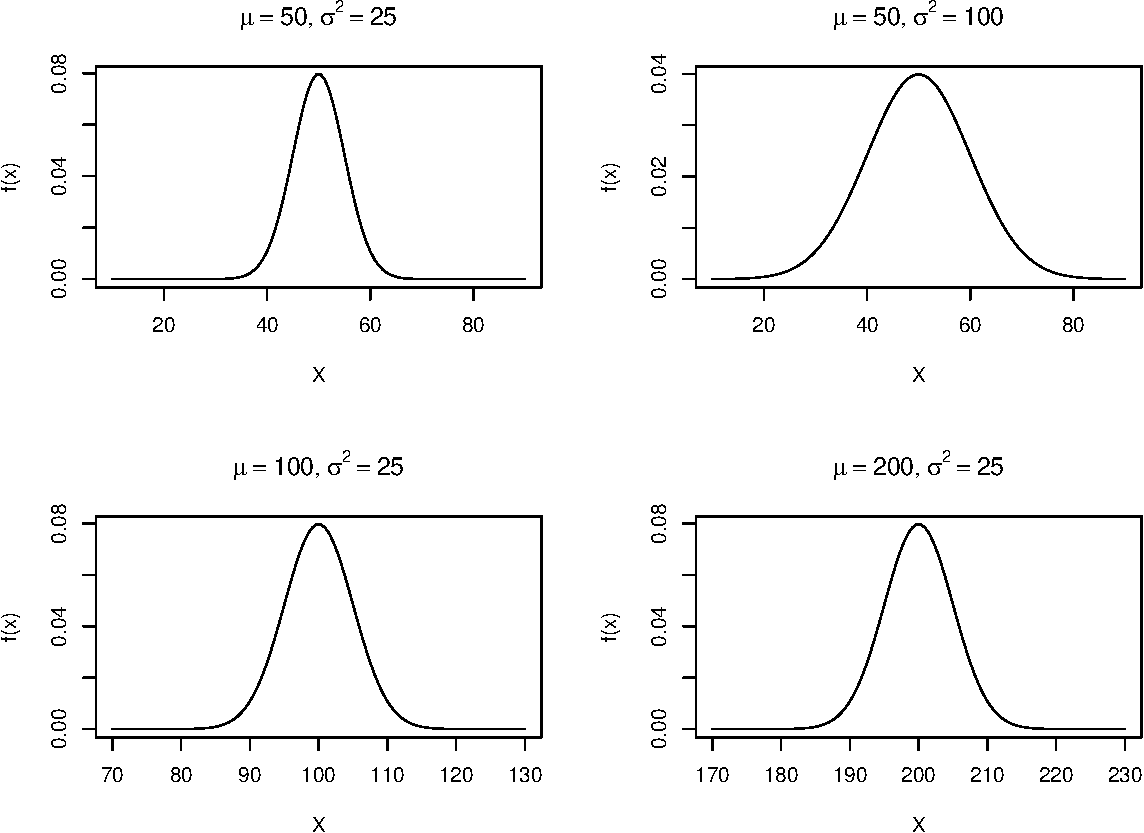
\includegraphics[width=1\textwidth]{figure/unnamed-chunk-5-1} 

}



\end{knitrout}
\end{frame}

\begin{frame}[fragile]{Modelo normal}
  \textbf{Característcas da curva normal:} \\~\\
  \begin{itemize}
  \item É \textbf{simétrica} em relação à $\mu$
  \item O ponto máximo (moda) de $f(x)$ é o ponto $x=\mu$
  \item Os pontos de inflexão da função são $\mu-\sigma$ e $\mu+\sigma$
  \item A área total sob a curva é 1 ou 100\%
  \item A curva é \textbf{assintótica} em relação ao eixo $x$
  \end{itemize}
\end{frame}

\begin{frame}[fragile]{Modelo normal}
  Para qualquer VA normal $X$, valem as seguintes relações: \\~\\
  \begin{align*}
    &P[X > \mu] = P[X < \mu] \\
    &P[\mu - \sigma < X < \mu + \sigma] \approxeq 0,6827 \\
    &P[\mu - 2\sigma < X < \mu + 2\sigma] \approxeq 0,9545 \\
    &P[\mu - 3\sigma < X < \mu + 3\sigma] \approxeq 0,9973
  \end{align*}
  Portanto, $6\sigma$ é frequentemente referida como a \textbf{largura}
  de uma distribuição normal. \\~\\
  Métodos mais avançados de integração podem ser utilizados para mostrar
  que a área sob a função densidade de probabilidade normal de $-\infty
  < x < \infty$ é igual a 1.
\end{frame}

\begin{frame}[fragile]{Modelo normal}
  Para obter uma probabilidade do modelo normal, devemos calcular a área
  entre os pontos $a$ e $b$, ou seja,
  \begin{equation*}
    P[a < X < b] = \int_a^b \frac{1}{\sqrt{2\pi}\sigma} \exp\left[-\frac{1}{2}
      \left( \frac{x - \mu}{\sigma}\right)^2\right] dx
  \end{equation*}
  No entanto, a função da distribuição normal não possui forma
  fechada, portanto o cálculo de probabilidades não pode ser feito
  diretamente pela integral, apenas por aproximações numéricas. \\~\\
  Para contornar esse problema, os valores de probabilidade são
  obtidos para uma distribuição normal padrão ($Z$) com $\mu = 0$ e
  $\sigma^2 = 1$,
  \begin{equation*}
    Z = \frac{X - \mu}{\sigma} \sim \text{N}(0,1)
  \end{equation*}
  que é o escore $Z$ (número de desvios-padrões da média $\mu$). A
  vantagem é que podemos fazer uma única tabela com as integrais
  aproximadas de $Z$, ao invés de uma tabela para cada par
  $(\mu,\sigma^2)$.
\end{frame}

\begin{frame}[fragile]{Modelo normal}
  Se $Z \sim \N(0,1)$, então sua fdp é
  \begin{equation*}
    f(z) = \frac{1}{\sqrt{2\pi}} \exp\left[-\frac{1}{2} (z)^2 \right]
  \end{equation*}
  Para se obter a probabilidade de $Z$ estar entre $a$ e $b$,
  \begin{equation*}
    P[a < Z < b] = \int_a^b \frac{1}{\sqrt{2\pi}} \exp\left[-\frac{1}{2}
      (z)^2 \right] dz
  \end{equation*}
  As integrais (áreas) para valores de $Z$ entre 0,00 e 3,99 estão na
  tabela. Portanto, para qualquer valor de $X$ entre $a$ e $b$, podemos
  calcular a probabilidade correspondente através da transformação,
  \begin{equation*}
    P[a < X < b] = P\left[\frac{a - \mu}{\sigma} < Z < \frac{b
        - \mu}{\sigma}\right]
  \end{equation*}
\end{frame}

\begin{frame}[fragile]{Modelo normal}
\begin{knitrout}\footnotesize
\definecolor{shadecolor}{rgb}{0.969, 0.969, 0.969}\color{fgcolor}

{\centering 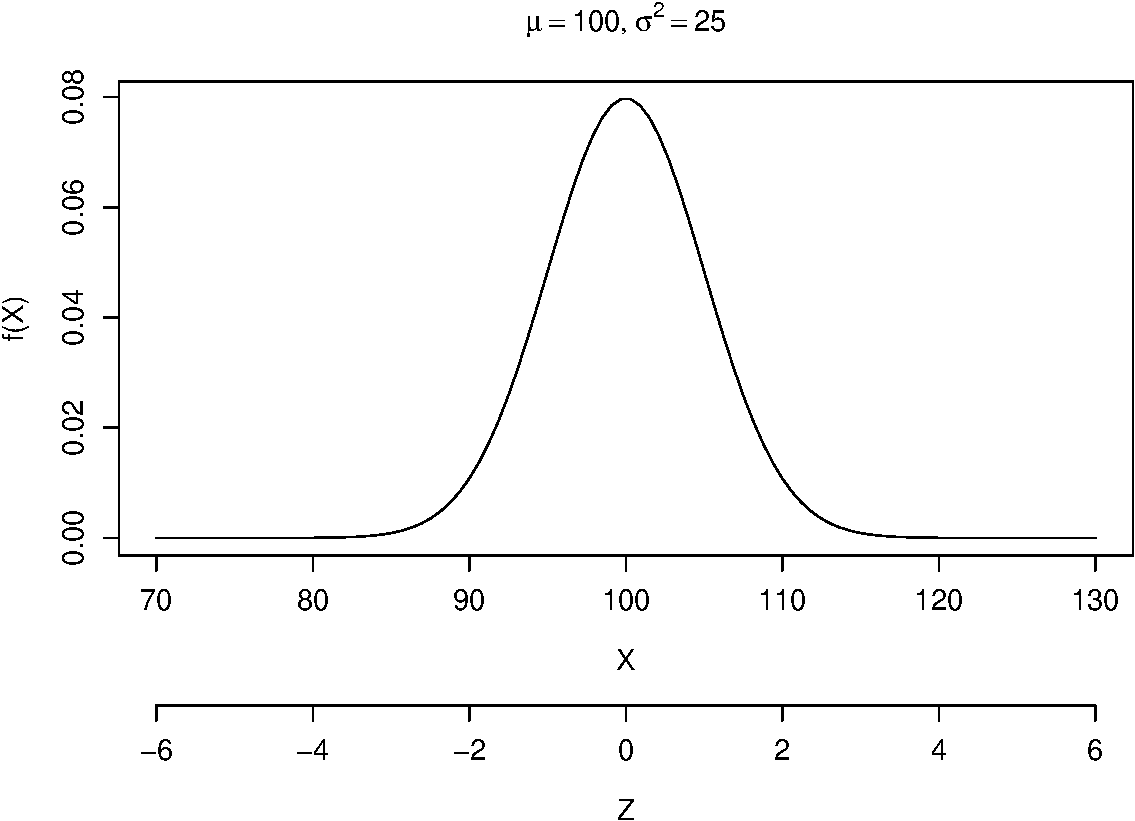
\includegraphics[width=1\textwidth]{figure/unnamed-chunk-6-1} 

}



\end{knitrout}
\end{frame}

\begin{frame}[fragile]{Modelo normal}
  \textbf{Exemplo de uso da tabela:} \\~\\
  Calcule as probabilidades (áreas):
  \begin{itemize}
  \item $P(0 < Z < 2)$
  \item $P(Z > 2)$
  \item $P(Z < -2)$
  \item $P(2,0 < Z < 2,5)$
  \item $P(-2,61 < Z < 2,43)$
  \item $P(Z > -1,63)$
  \end{itemize}
\end{frame}

\begin{frame}[fragile]{Modelo normal}
  \textbf{Exemplos} \\~\\
  \begin{enumerate}
  \item Suponha que a média populacional do coeficiente de inteligência
    (QI) seja 100, com desvio-padrão 15. Qual a probabilidade de
    selecionarmos uma pessoa ao acaso, e ela ter QI entre 90 e 115?
  \item Seja $X \sim \N(30, 16)$. Qual a probabilidade de obtermos um
    valor maior ou igual a 38?
  \end{enumerate}
\end{frame}

\begin{frame}[fragile]{Modelo normal}
  \textbf{Exemplo:} A duração de um pneu de automóvel, em quilômetros
  rodados, apresenta distribuição normal com média 70000 km, e
  desvio-padrão de 10000 km. Com isso:
  \begin{itemize}
  \item[(a)] Qual a probabilidade de um pneu escolhido ao acaso durar mais de
    85000 km?
  \item[(b)] Qual a probabilidade de um pneu durar entre 68500 km e 75000 km?
  \item[(c)] Qual a probabilidade de um pneu durar entre 55000 km e 65000 km?
  \item[(d)] O fabricante deseja fixar uma garantia de quilometragem, de tal
    forma que, se a duração de um pneu for inferior à da garantia, o
    pneu será trocado. De quanto deve ser essa garantia para que somente
    1\% dos pneus sejam trocados?
  \item[(e)] De acordo com o item anterior, a probabilidade de que um pneu
    seja trocado é de 1\%. Se o fabricante vende 5000 pneus por mês,
    quantos pneus deve trocar?
  \end{itemize}
\end{frame}

\section{Exercícios}

\begin{frame}[fragile]{Exercícios}
  \begin{itemize}
  \item Montgomery, DC; Runger, GC. \textbf{Estatística aplicada e
      probabilidade para engenheiros}. Rio de Janeiro: LTC Editora,
    2012.
    \begin{itemize}
    \item Cap. 3: 14--17, 21, 26--28, 47--51, 60, 78, 79, 85--87, 90,
      98, 129--132, 135, 141, 142.
    \item Cap. 4: 2, 4, 5, 7, 27--30, 33, 53, 55, 61, 69, 70, 75.
    \end{itemize}
  \end{itemize}
\end{frame}

\section{Referências}

\begin{frame}{Referências}
  \begin{itemize}
  \item Bussab, WO; Morettin, PA. \textbf{Estatística básica}. São
    Paulo: Saraiva, 2006. [Cap. 6]
  \item Magalhães, MN; Lima, ACP. \textbf{Noções de Probabilidade e
      Estatística}. São Paulo: EDUSP, 2008. [Cap. 3]
  \item Montgomery, DC; Runger, GC. \textbf{Estatística aplicada e
      probabilidade para engenheiros}. Rio de Janeiro: LTC Editora,
    2012. [Cap. 3 e 4]
  \end{itemize}
\end{frame}




\end{document}
